\documentclass[../../main.tex]{subfiles}

\begin{document}

Using recurrent structures such as RNNs
was the dominant strategy in sequence modeling before transformer networks.
Every sentence token was represented as a hidden state
that is a function of all previous hidden states.
While this approach has a reasonable motivation,
the sequential nature contraints computation speed for a single training example.
This limitation is especially hindering for longer sequences,
where batching the training data is only possible to a memory limit.
Attempts to minimize sequential computation included using convolutional networks
that can be computed in parallel.
For these models however,
the number of operations required to relate two tokens
grows in the distance of their positions in the sequence.
Attention mechanisms allow modeling token relationships
independent of their distance in a sequence.

\begin{figure}[t]
    \centering
    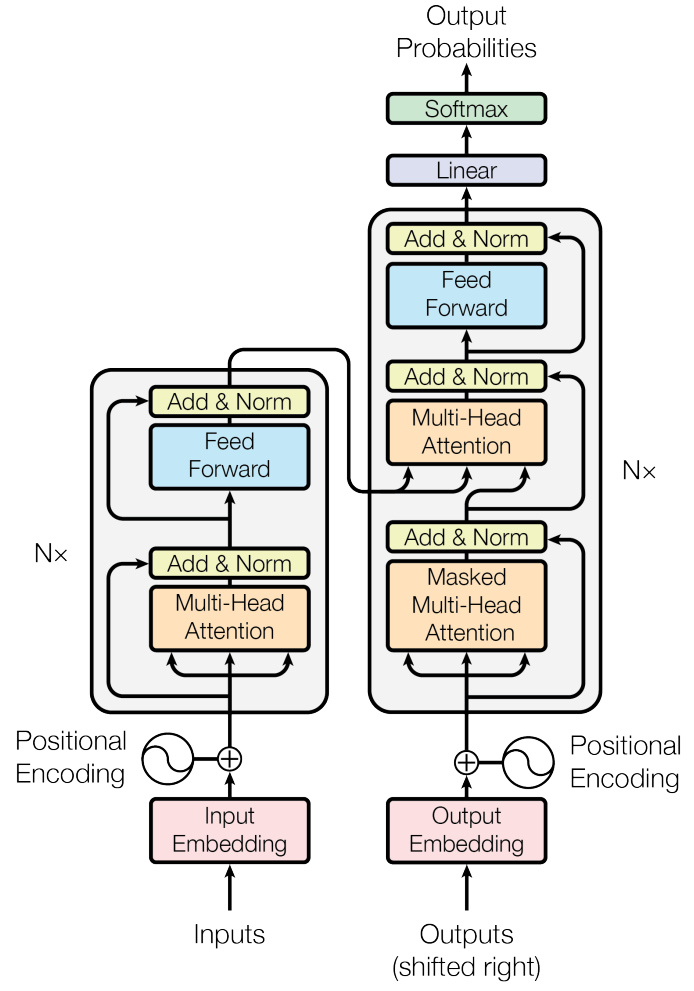
\includegraphics[scale=0.4]{include/images/transformer_architecture.png}
    \caption{
        The encoder-decoder architecture
        of a full transformer network \cite{Vaswani2017}.
        The encoder (left) can attend over all positions to learn rich embeddings.
        The decoder (right) can generate output sequences.
        The first decoder attention layer
        can only attend on previous position of the input sequence,
        while the second can attend over the outputs of the encoder.
        This combines a sequence-to-sequence with
        auto-regressive properties into the decoder.
    }
    \label{fig:transformer_arch}
\end{figure}

The transformer network \cite{Vaswani2017}
shown in Figure \ref{fig:transformer_arch}
was the first model that removes all recurrent structures
and only relys on attention mechanisms.
In particular,
they use multi-headed self-attention layers.
Attention mechanisms learn dependencies between tokens in sentences
without regard to their distance.
Their non-sequential charactericstics allow for better parallelization.
Self-attention is an attention mechanism
that computes relations between different positions of the same sequence
with the goal of finding a representation of the sequence.

Since the transformer architecture does not use any recurrent structures,
the order of the tokens in the sequence must be manually injected.
Positional encodings are added to the input embeddings to achieve this.

Like most language modeling networks,
a transformer consists of an enconder and a decoder.
The encoder has two sub-layers,
a multi-head attention block
and a fully connected feed foward block.
The decoder is similar to the encoder
but has an additional multi-head attentention layer
that attends on the outputs of the encoder.
The first attention layer is masked
and the decoder input sequence is shifted by right,
so only previous positions can be
attended by the decoder.

The full architecture has capabilites of a classic sequence-to-sequence model
used for tasks like language translation.
All positions in the decoder can attend over all positions in the encoder.
For other tasks however,
the individual encoder and decoder sections are a better fit,
as explained in the sections \ref{subsec:embedding} and \ref{subsec:gpt}.

\end{document}